%%%--------------------------------%%%
%%% UC4
%%%--------------------------------%%%
\newpage
% UC4 ====================================================
\subsubsection{Use Case Specification: \ac{UC}4 Project risk adjustment}
\label{sec:domainBbe}

\paragraph*{Description}\mbox{}\\
After a risk has been submitted and evaluated by the team it is grouped into three categories. However, within these categories the initial order is simply that the risks submitted first will be placed at the top. This use case allows the teams to prioritize risks according to their perceived risk urgency. On the project risk overview page the after the initial risk evaluation users will find a button they can use to adjust the ranking. They will then enter adjustment mode where they can arrange the risks according to their perceived urgency and submit their ranking. Then they will return to the overview where the risks will be displayed according to their average relative ranking positions. The adjust button will be disabled until new risks are added to prevent manipulation. The user will be notified that they cannot rank multiple times when they first go through the adjustment process. 

\paragraph*{Screenshots}\mbox{}\\
tbd: Insert screenshots and shortly explain what can be seen

\begin{figure}[h] 
	\centering
	
\includegraphics[width=0.1\textwidth]{Content/Domain/placeholder.png}
	\caption{Use Case X: Detail}
	\label{fig:label4}
\end{figure}

\paragraph*{Basic Flow} \mbox{}\\
\begin{itemize}
	\vspace{-3mm}
	\setlength\itemsep{-1em}
	\item The user is on the project overview site with all project risks.
	\item By clicking on a "Rank Risks" button the ranking view is enabled and the button becomes a submit button.
	\item The user can order the risks according to his personal priority.
	\item The user submits their preferred order.
	\item This order is submitted to the server and the average rank for every risk according to the current submissions is calculated.
	\item The risks on the risk overview page are displayed accordingly.
	\item The adjust button is disabled for users who have already submitted a ranking.
\end{itemize}

\subparagraph{Activity Diagram}\mbox{}\\
\begin{figure}[H]
	\centering
	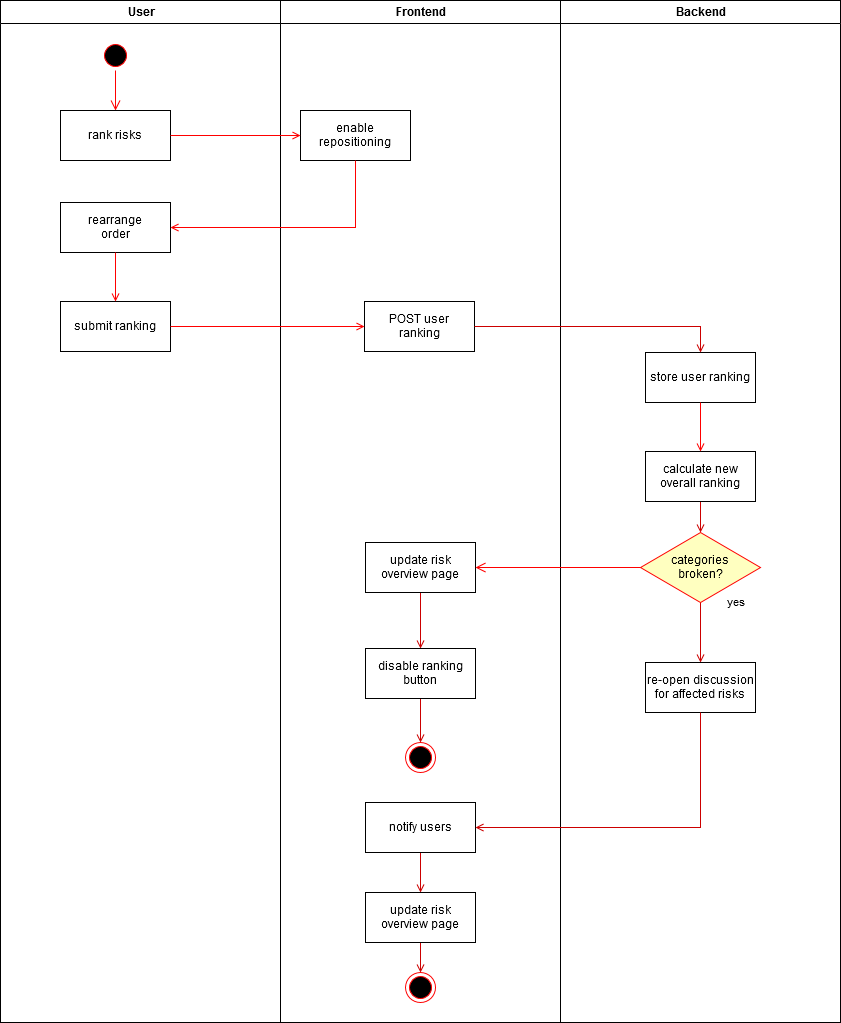
\includegraphics[width=0.8\textwidth]{Content/Domain/UC4RiskAdjustmentDiagram.png}
	\caption{Activity Diagram Use Case 4}
	\label{fig:label44}
\end{figure}

\paragraph*{Alternative Flows}\mbox{}\\

The following steps will be added if the user enters the ranking process for the first time or has not participated in a ranking process for a prolonged period of time:
\begin{itemize}
	\vspace{-3mm}
	\setlength\itemsep{-1em}
	\item When the user presses the ranking button before the ranking mode is enabled an explation prompt will be shown.
	\item The user will be informed that they can submit their ranking only once.
	\item The user can either choose to confirm or they can choose that they do not want to be notified again doubling the time before the notification is shown again.
\end{itemize}

The following steps will be added should the risk adjustment contradict the intital risk assesment:
\begin{itemize}
	\vspace{-3mm}
	\setlength\itemsep{-1em}
	\item A risk is ranked outside its category due to the average ranking process.
	\item The risk discussion on the risks which are now out of category is re-opened.
	\item The team members receive a notification to re-evaluate those risks.
\end{itemize}


\paragraph*{Special Requirements and Preconditions}\mbox{}\\
This use case has the following preconditions:
\begin{enumerate}
	\vspace{-3mm}
	\setlength\itemsep{-1em}
	\item The user is part of a project which contains risks.
	\item The initial risk discussion is finished.
	\item The user has either not yet ranked the risks or 
	\item the risk adjustment has been re-opened by the project manager.
\end{enumerate}

\paragraph*{Postconditions and Persistance}\mbox{}\\
The postconditions for this use case are:
\begin{enumerate}
	\vspace{-3mm}
	\setlength\itemsep{-1em}
	\item The risk order will be updated for all project members.
	\item The ranking option will be disabled until new risks are proposed or the ranking is manually reset by the project manager.
	\noindent	
	The ranking results are persisted in the database. The user ranking is transmitted to the backend via post request where the project risk ranking is handled accordingly.
\end{enumerate}